\begin{figure}[h!]
    \centering
    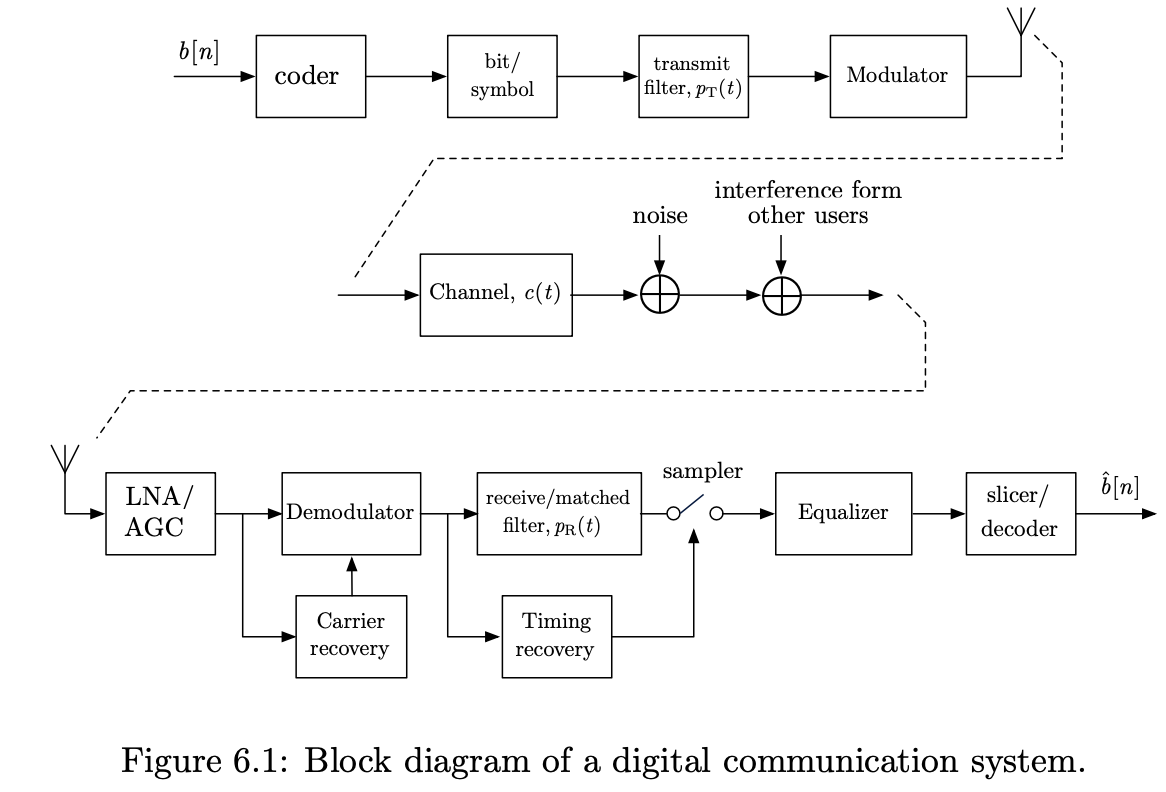
\includegraphics[scale=0.7]{figures/software_radio_system.png}
    \caption{Block Diagram of A Communications System}
    \label{fig:comm-system}
\end{figure}
\begin{figure}[h!]
    \centering
    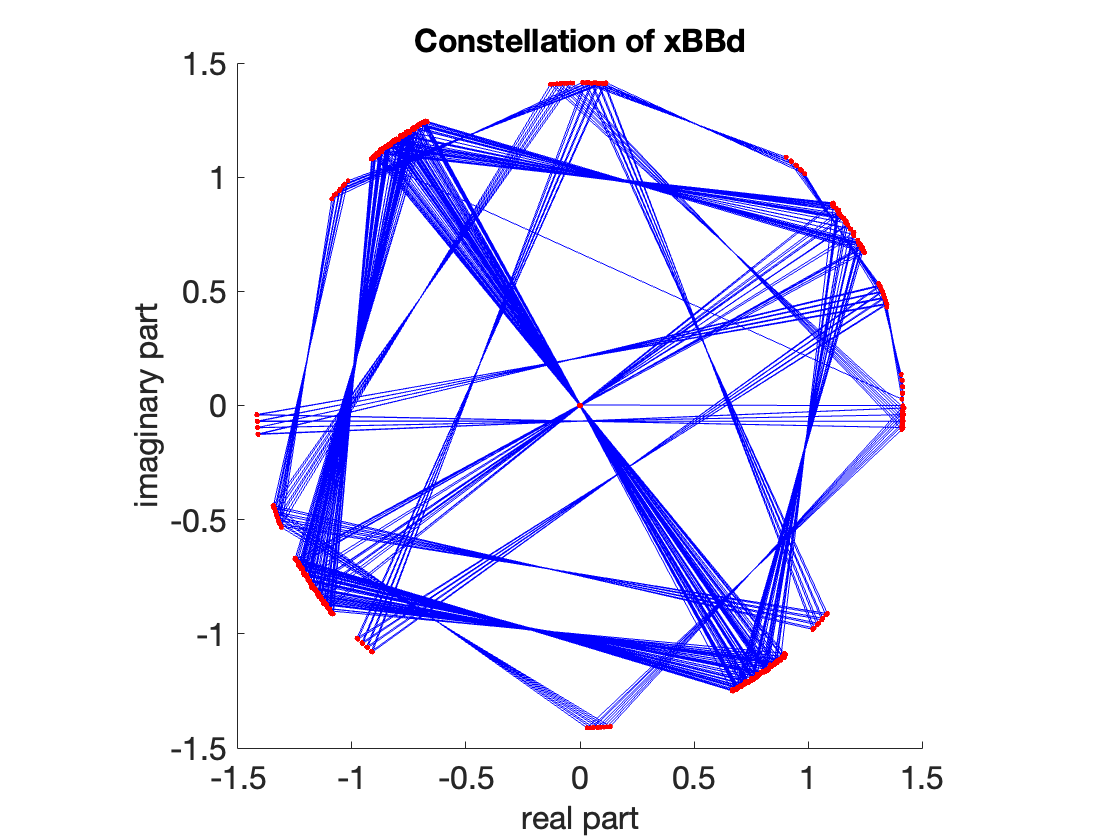
\includegraphics[scale=0.5]{figures/constellation_rotation.png}
    \caption{Result of Frequency Offset in QPSK Constellation}
    \label{fig:qpsk-rotate}
\end{figure}
\begin{figure}[h!]
    \centering
    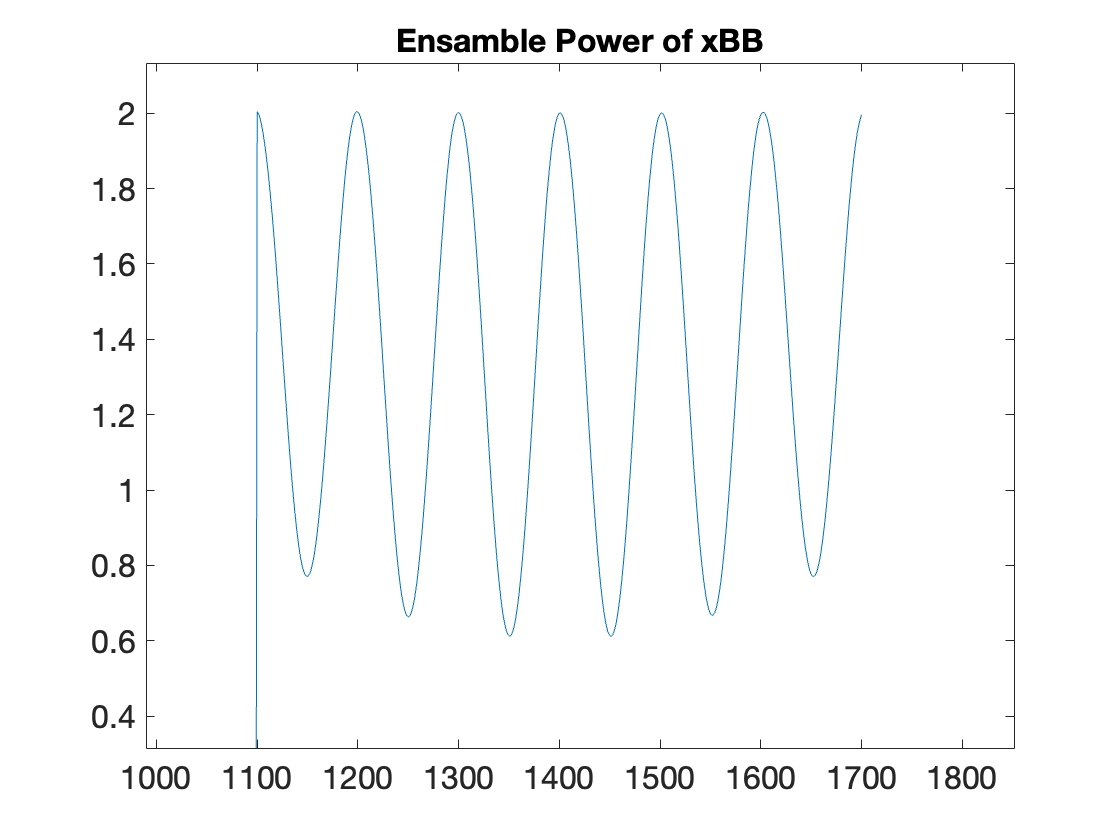
\includegraphics[scale=0.5]{figures/ensemble_power.png}
    \caption{Ensemble Power of xRF1.mat}
    \label{fig:ensemble-power}
\end{figure}
\begin{figure}[h!]
    \centering
    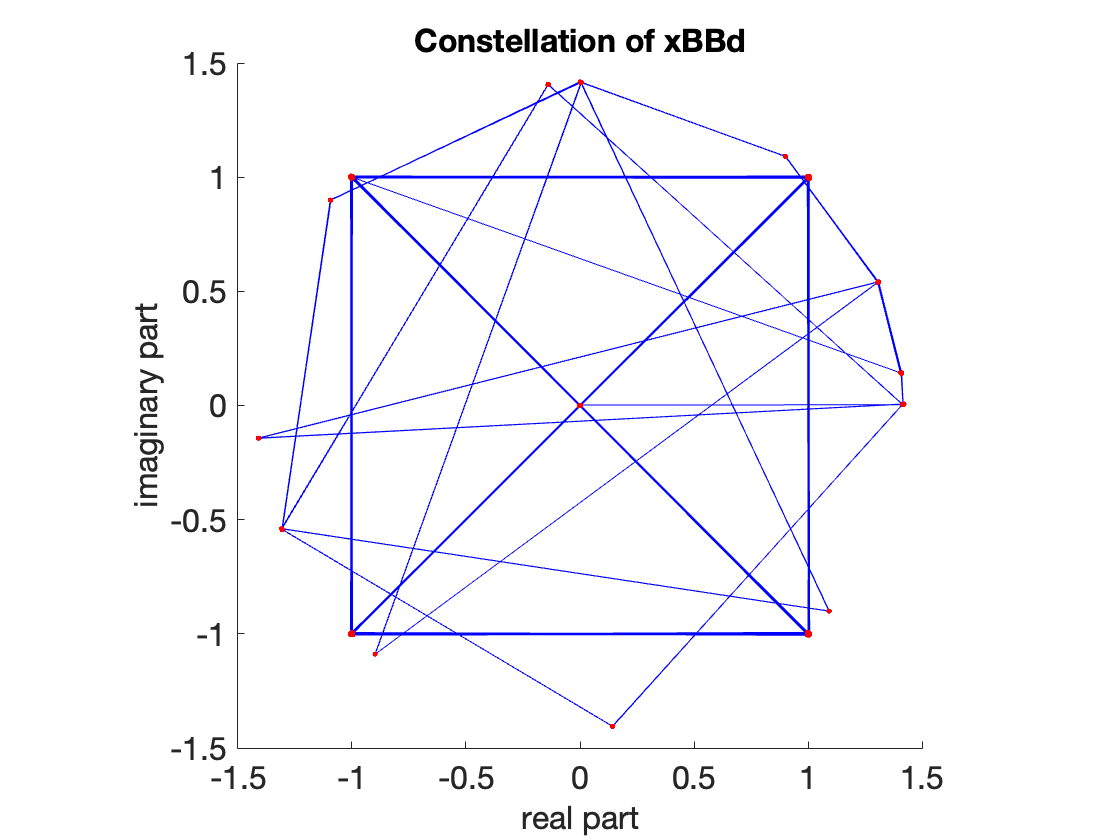
\includegraphics[scale=0.5]{figures/packet_qpsk_constellation.png}
    \caption{Packet QPSK Constellation of xRF1.mat}
    \label{fig:parti-packet-constellation}
\end{figure}
\begin{figure}[h!]
    \centering
    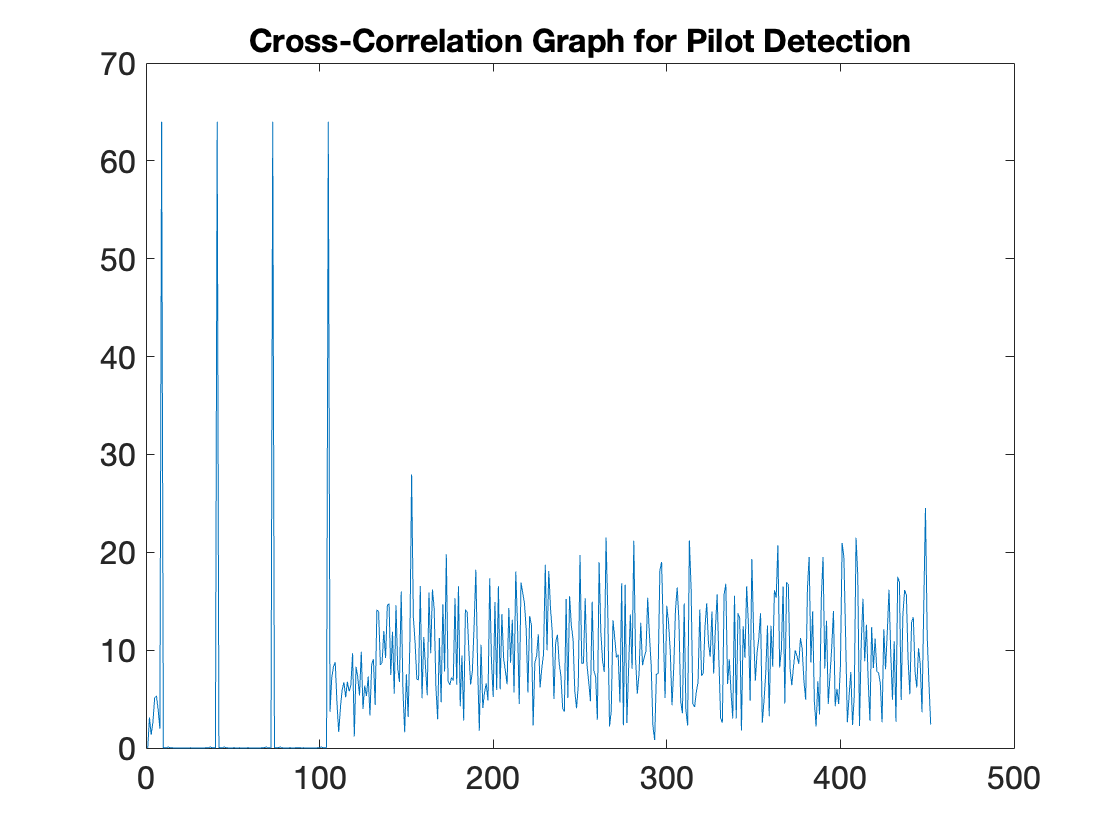
\includegraphics[scale=0.5]{figures/cross-correlation-parti.png}
    \caption{Cross-Correlation of Premable with Pilot of xRF1.mat}
    \label{fig:cross-corr-parti}
\end{figure}
\begin{figure}[h!]
    \centering
    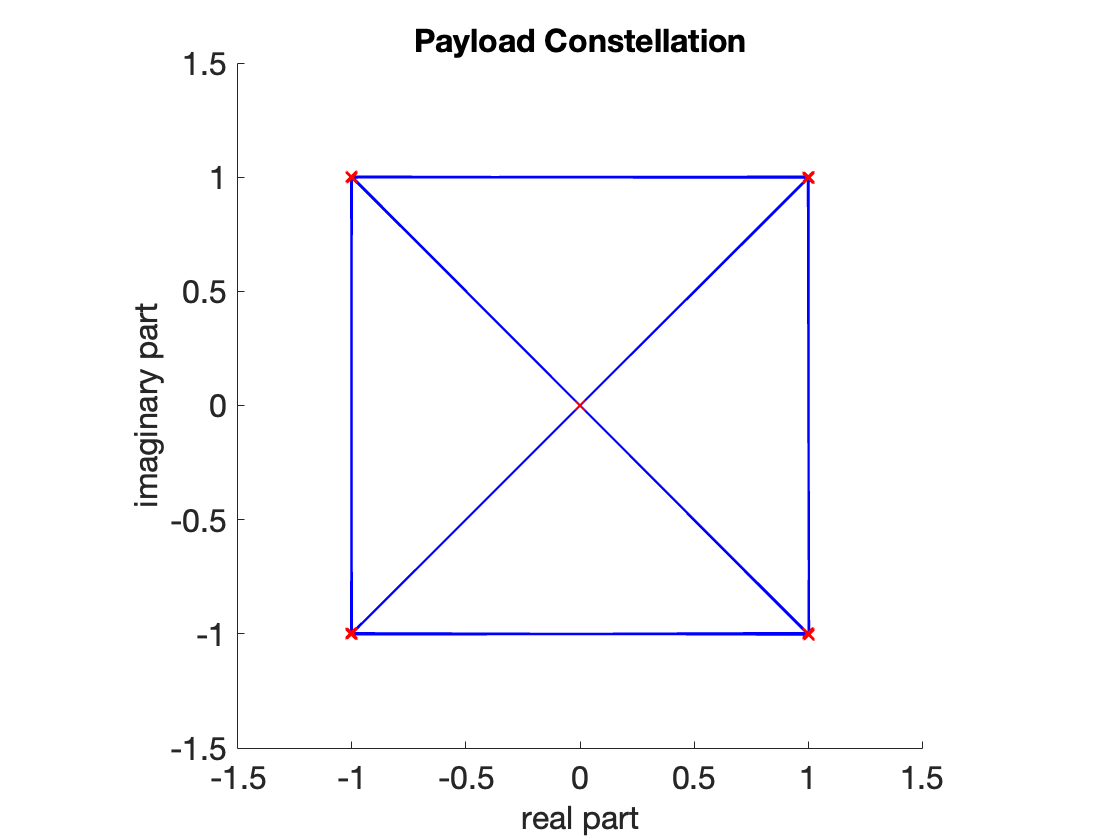
\includegraphics[scale=0.5]{figures/payload-constellation-parti.png}
    \caption{Payload QPSK Constellation of xRF1.mat}
    \label{fig:payload-constellation-parti}
\end{figure}
\begin{figure}[h!]
    \centering
    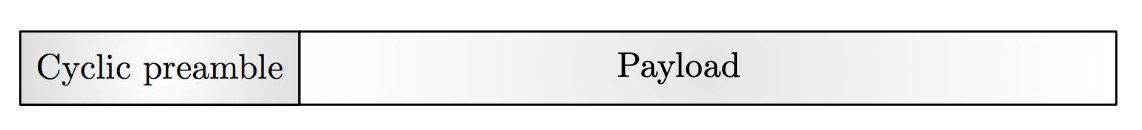
\includegraphics[scale=0.7]{figures/data_sequence.png}
    \caption{Structure of transmitted packets in project}
    \label{fig:data_sequence}
\end{figure}
\begin{figure}[h!]
    \centering
    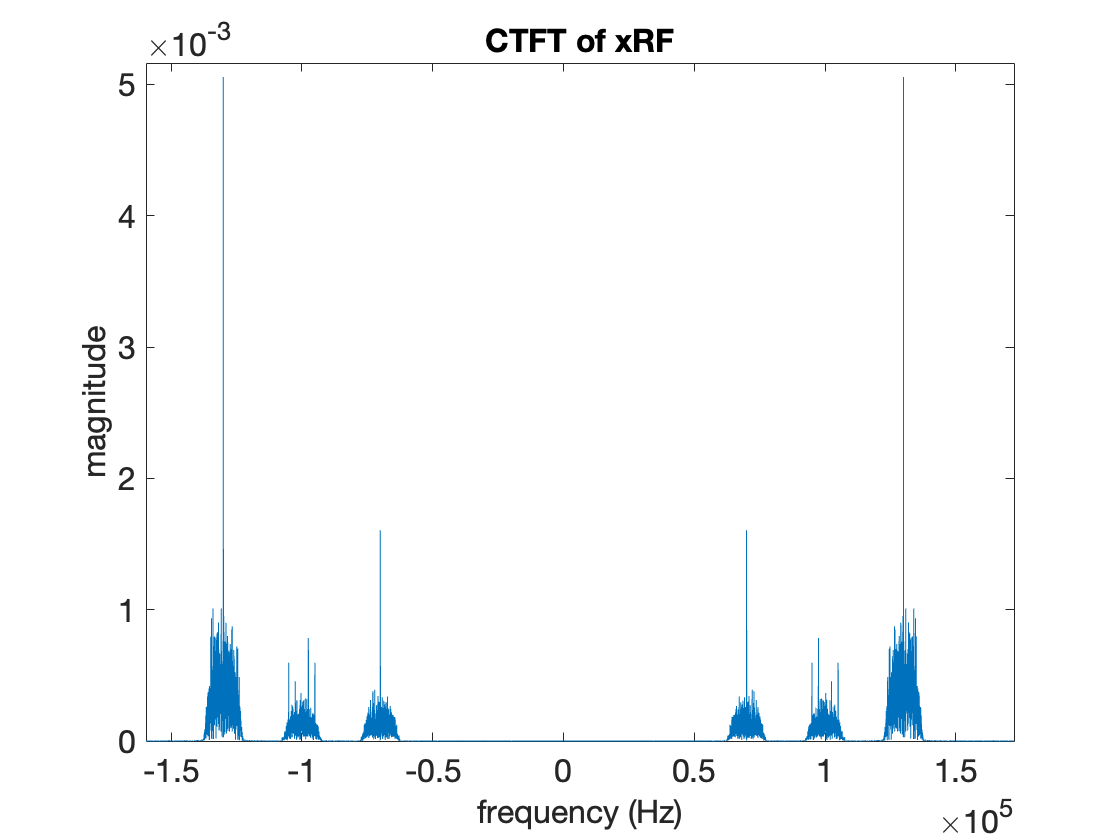
\includegraphics[scale=0.4]{figures/xRF1 spectrum.png}
    \caption{Spectrum of xBB signal in Part I}
    \label{fig:xbb_partI}
\end{figure}
\begin{figure}[h!]
    \centering
    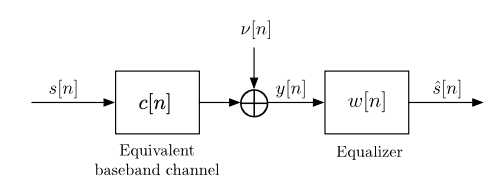
\includegraphics[scale=1.5]{figures/discrete_time_symbol_spaced.png}
    \caption{Discrete Time Symbol-Spaced Equalizer}
    \label{fig:symbol-spaced}
\end{figure}
\begin{figure}[h!]
    \centering
    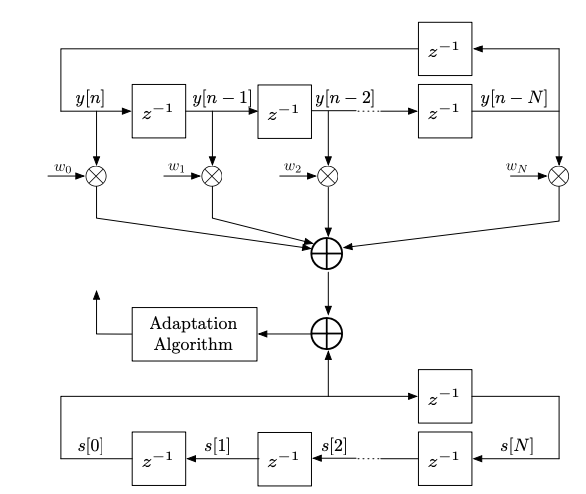
\includegraphics[scale=1]{figures/symbol_spaced_cyclic.png}
    \caption{Symbol-Spaced Cyclic Equalizer Training}
    \label{fig:symbol-cyclic}
\end{figure}
\begin{figure}[h!]
    \centering
    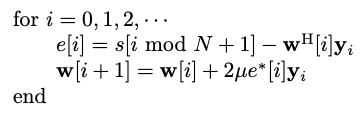
\includegraphics[scale=1]{figures/equalizer code.png}
    \caption{Cyclic Symbol-Spaced Equalizer Code}
    \label{fig:symbol-code}
\end{figure}
\begin{figure}[h!]
    \centering
    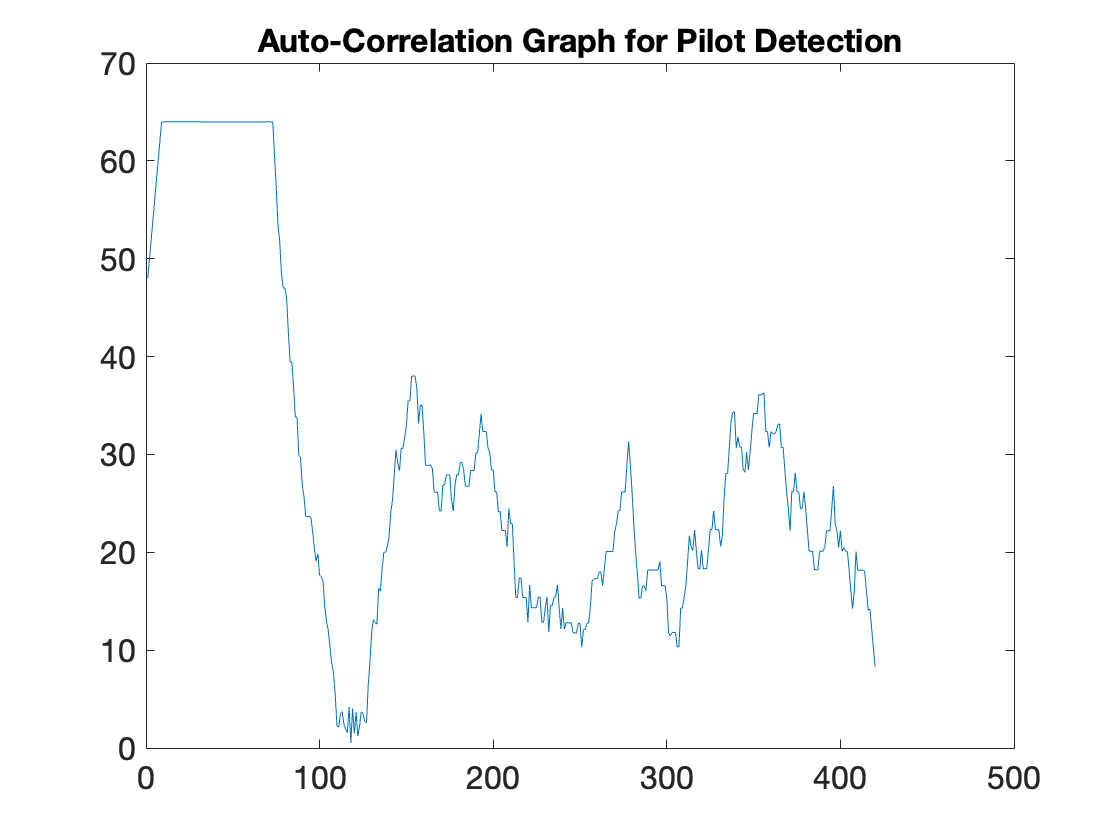
\includegraphics[scale=0.4]{figures/auto-correlation.png}
    \caption{Auto-correlation to Find Preamble on xRF1.mat}
    \label{fig:auto-corr}
\end{figure}
\begin{figure}[h!]
    \centering
    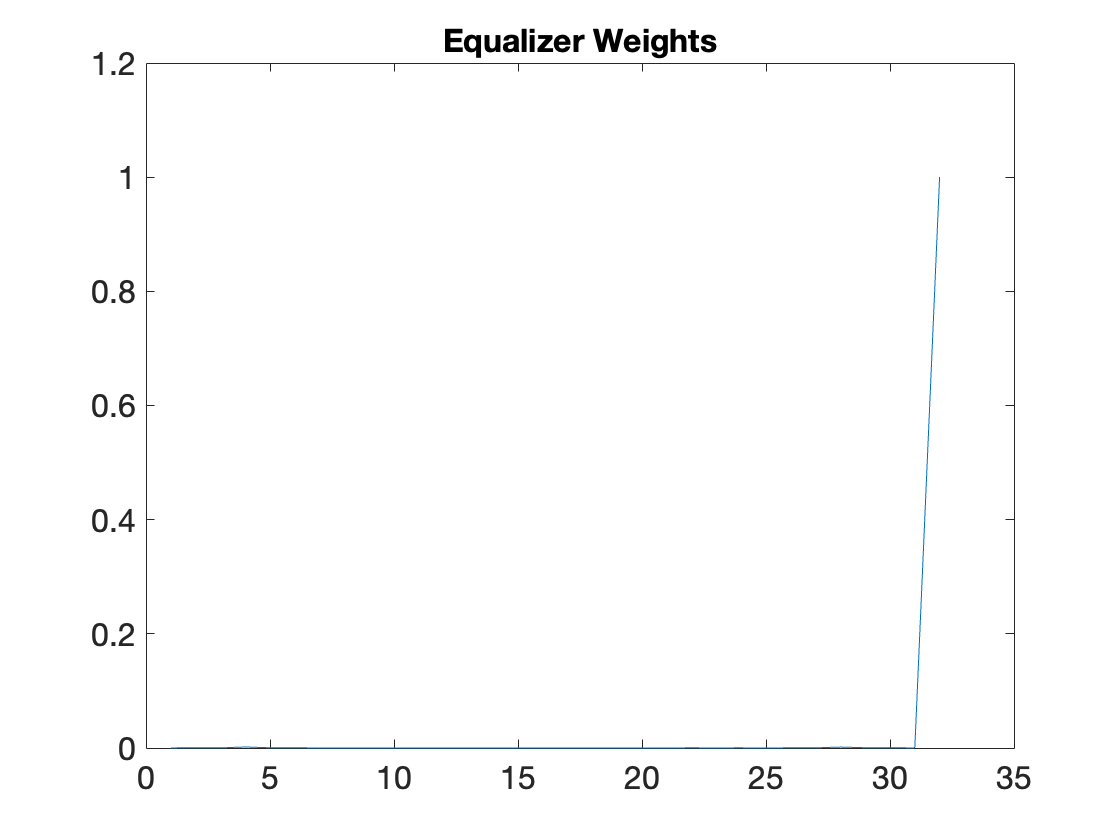
\includegraphics[scale=0.4]{figures/non_shifted_weights.png}
    \caption{Non-Shifted Tap-Weights of Symbol-Spaced Equalizer on xRF1.mat}
    \label{fig:non-circ-weights}
\end{figure}
\begin{figure}[h!]
    \centering
    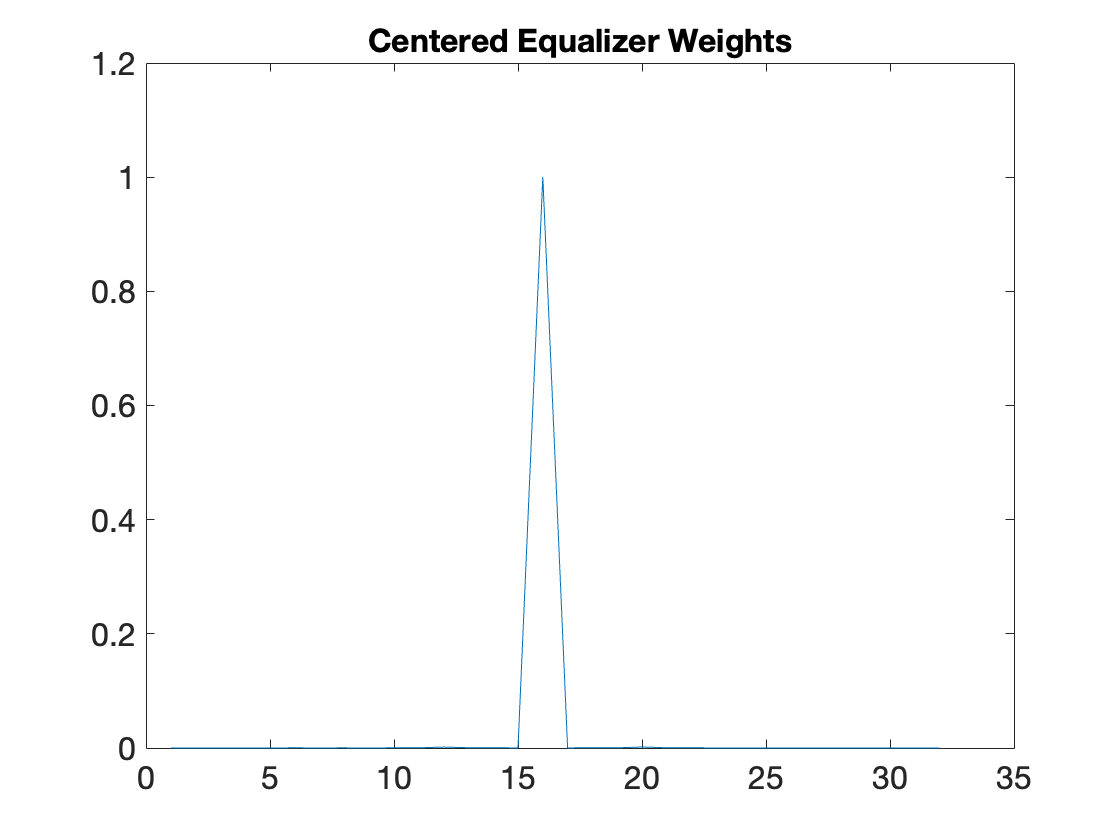
\includegraphics[scale=0.4]{figures/shifted_tap_weights.png}
    \caption{Shifted Tap-Weights of Symbol-Spaced Equalizer on xRF1.mat}
    \label{fig:circ-weights}
\end{figure}
\begin{figure}[h!]
    \centering
    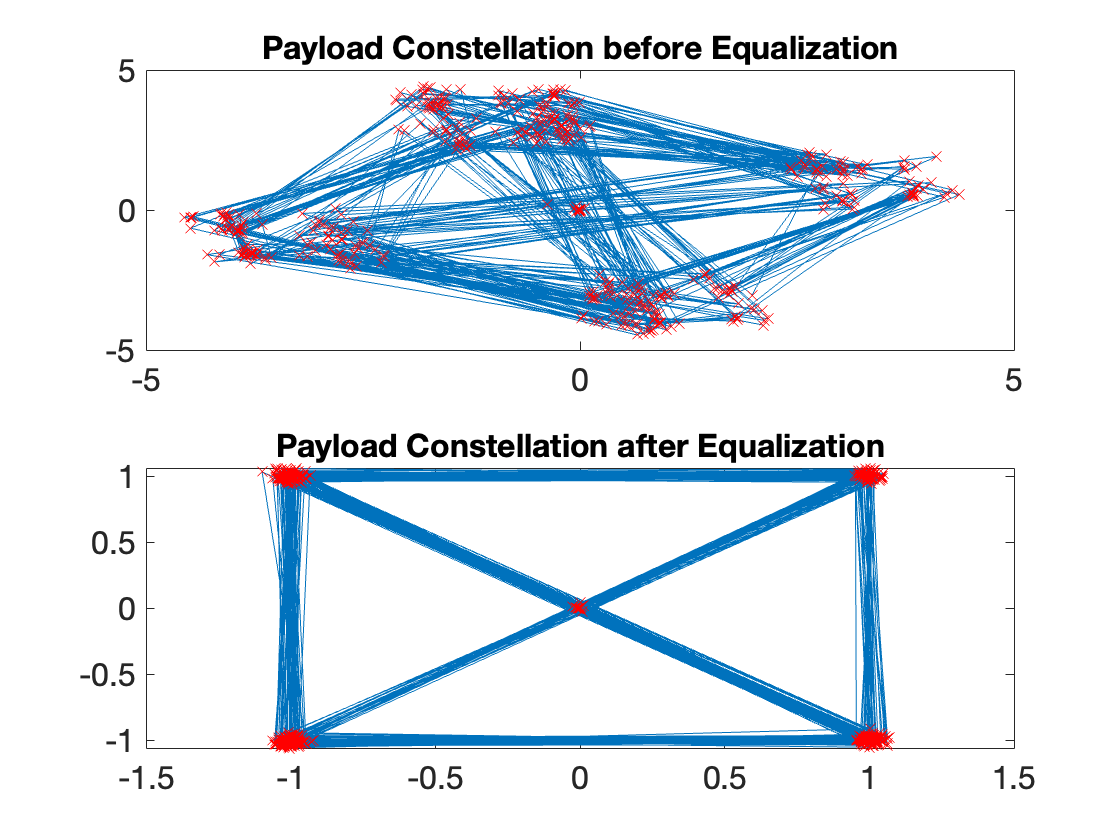
\includegraphics[scale=0.4]{figures/payload_equalization_part2.png}
    \caption{Payload Constellation of xRF3.mat before and after Symbol-Spaced Equalization}
    \label{fig:payload-equal-part2}
\end{figure}
\begin{figure}[h!]
    \centering
    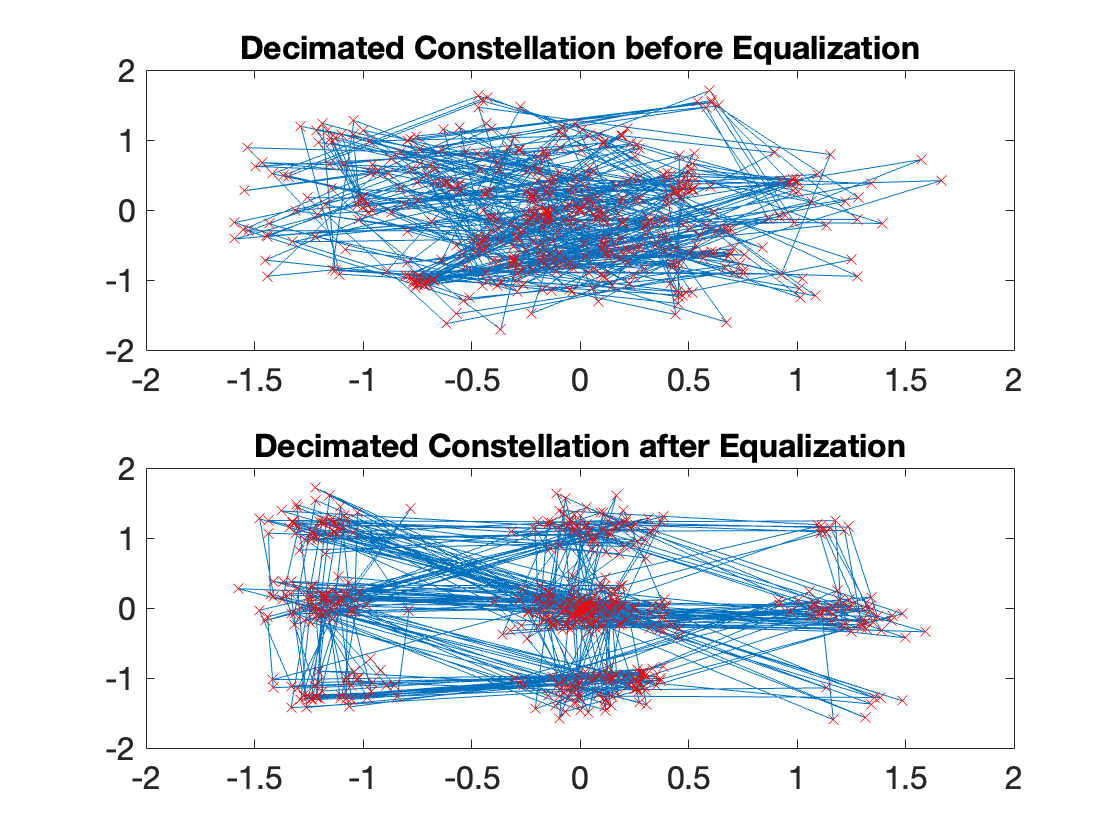
\includegraphics[scale=0.4]{figures/bad_timing_phase_part2.png}
    \caption{Payload Constellation of xRF5.mat before and after Symbol-Spaced Equalization with Wrong Timing Phase}
    \label{fig:payload-equal-wrong-phase-part2}
\end{figure}


\begin{figure}[h!]
    \centering
    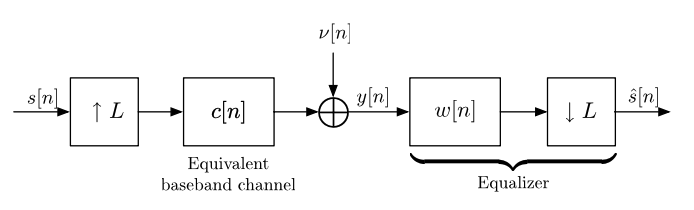
\includegraphics[scale=0.4]{figures/fractionally_spaced.png}
    \caption{Fractionally-Spaced Equalizer}
    \label{fig:frac-equal}
\end{figure}

\begin{figure}[h!]
    \centering
    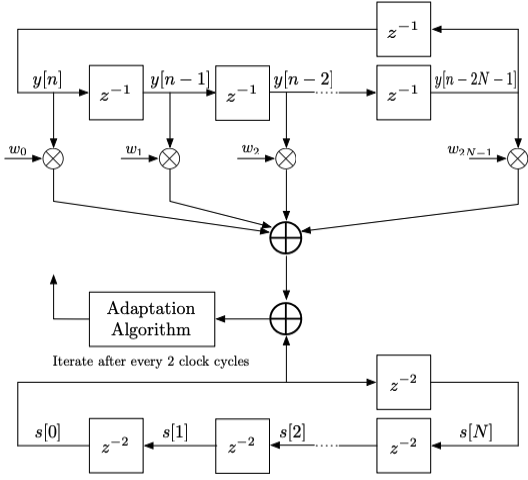
\includegraphics[scale=0.4]{figures/cyclic-frac.png}
    \caption{Fractionally-Spaced Cyclic Equalizer}
    \label{fig:cyclic-frac}
\end{figure}
\begin{figure}[h!]
    \centering
    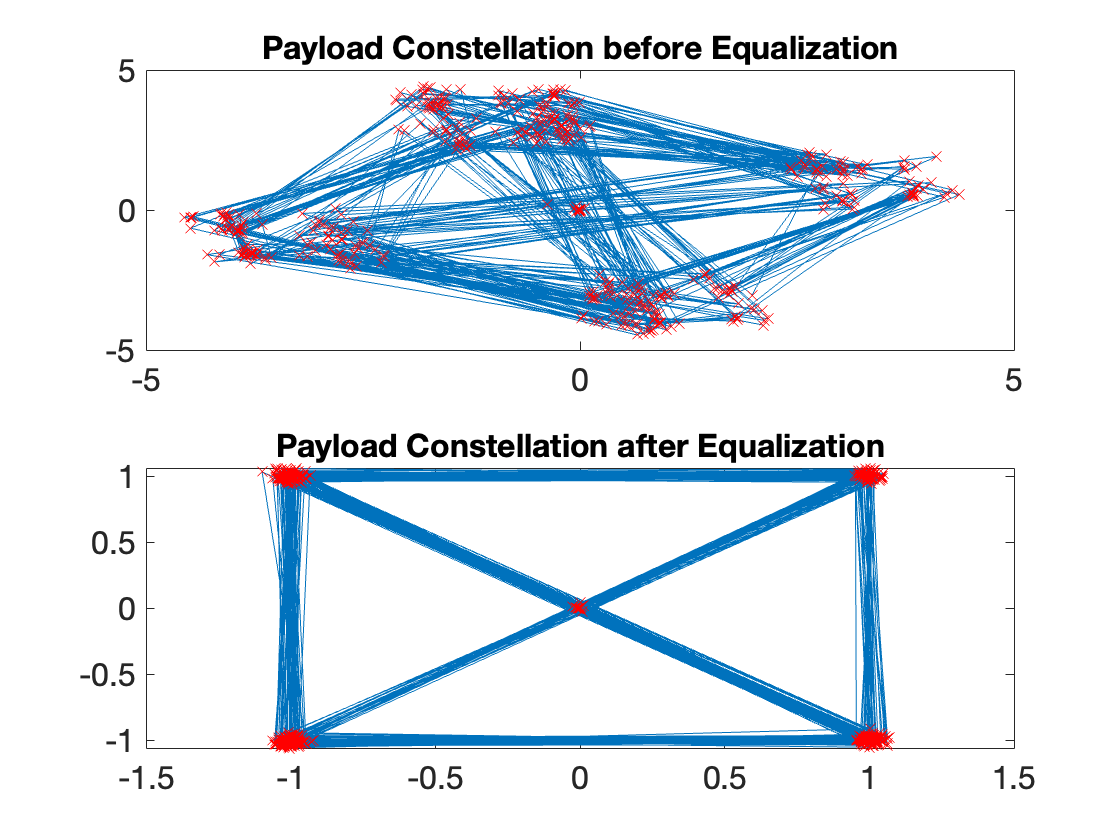
\includegraphics[scale=0.4]{figures/payload_constellation_part3.png}
    \caption{Payload Constellation of xRF3.mat before and after Half Symbol-Spaced Equalization}
    \label{fig:payload-equal-part3}
\end{figure}

\begin{figure}[h!]
    \centering
    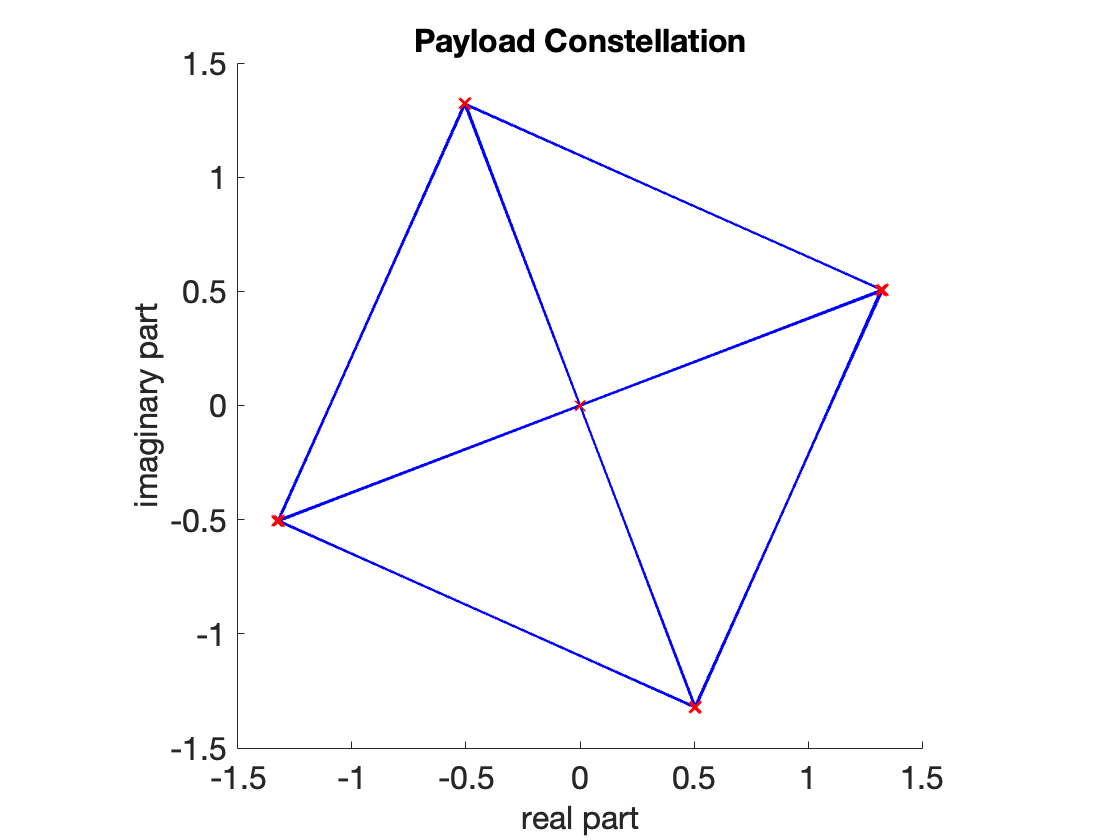
\includegraphics[scale=0.4]{figures/ideal-channel-carrier-phase.png}
    \caption{Ideal Channel xRF1.mat with Carrier Phase Offset}
    \label{fig:phase-rotate}
\end{figure}
\begin{figure}[h!]
    \centering
    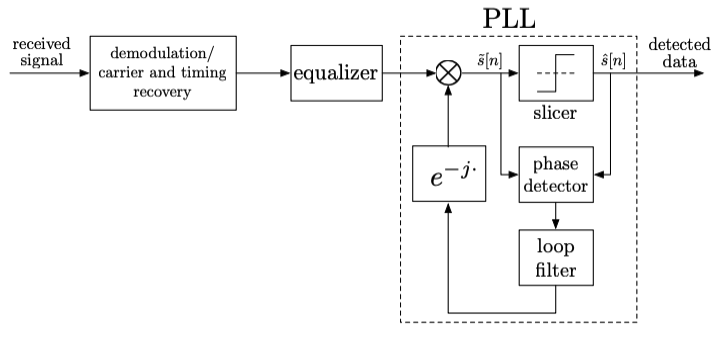
\includegraphics[scale=0.4]{figures/phase_pll.png}
    \caption{Data-Aided Phase PLL}
    \label{fig:phase-pll}
\end{figure}
\begin{figure}[h!]
    \centering
    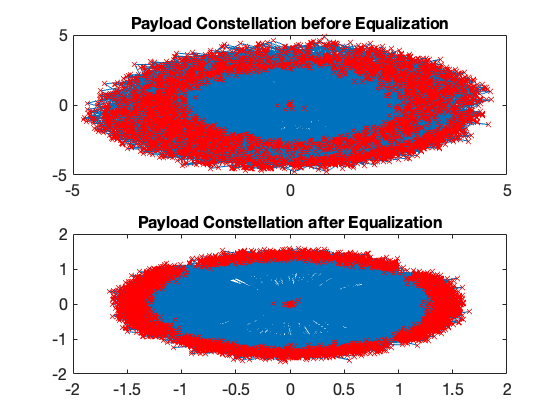
\includegraphics[scale=0.4]{figures/payload_xrf7_before_dd.png}
    \caption{Payload of xRF7.mat Before Decision Directed Carrier Phase Removal}
    \label{fig:before-dd}
\end{figure}
\begin{figure}[h!]
    \centering
    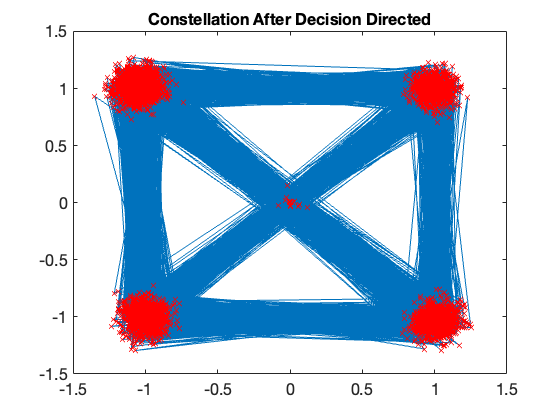
\includegraphics[scale=0.4]{figures/payload_xrf7_after_dd.png}
    \caption{Payload of xRF7.mat After Decision Directed Carrier Phase Removal}
    \label{fig:after-dd}
\end{figure}


\begin{figure}[h!]
    \centering
    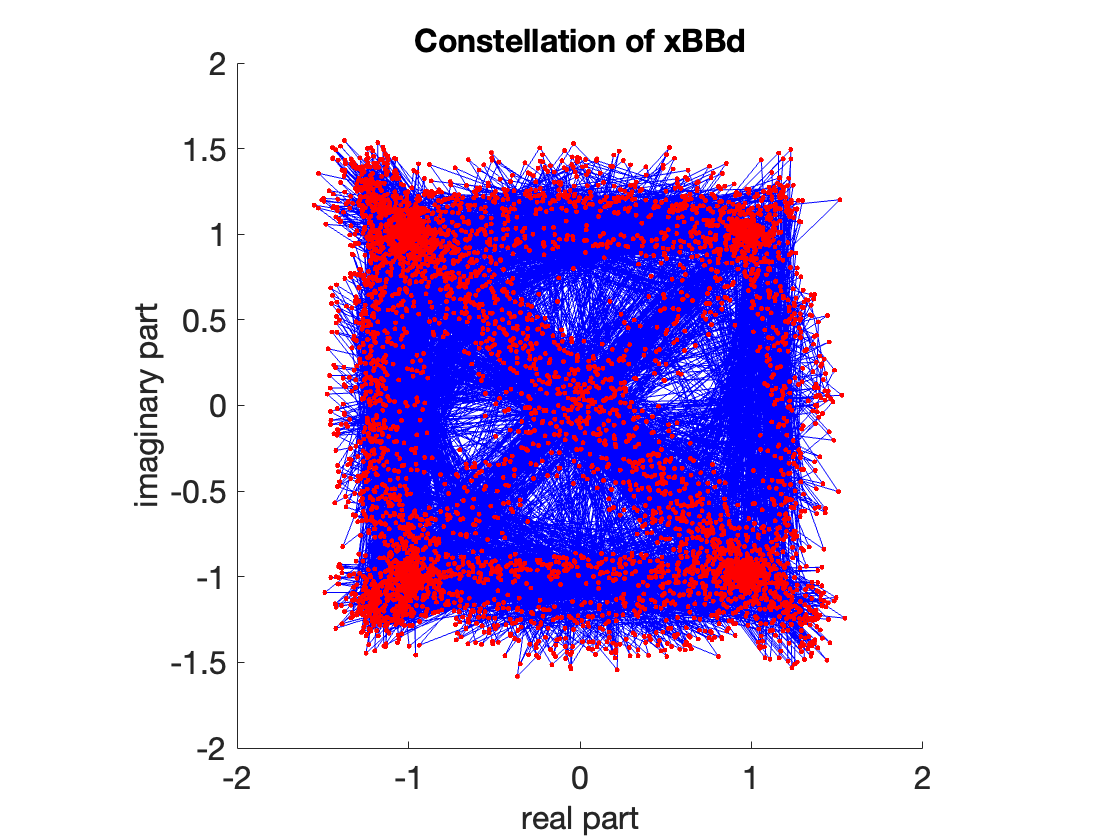
\includegraphics[scale=0.4]{figures/no-timing-phase-corr-xrf9.png}
    \caption{Payload of xRF9.mat No Decision Directed Timing Phase Recovery}
    \label{fig:no-dd}
\end{figure}
\begin{figure}[h!]
    \centering
    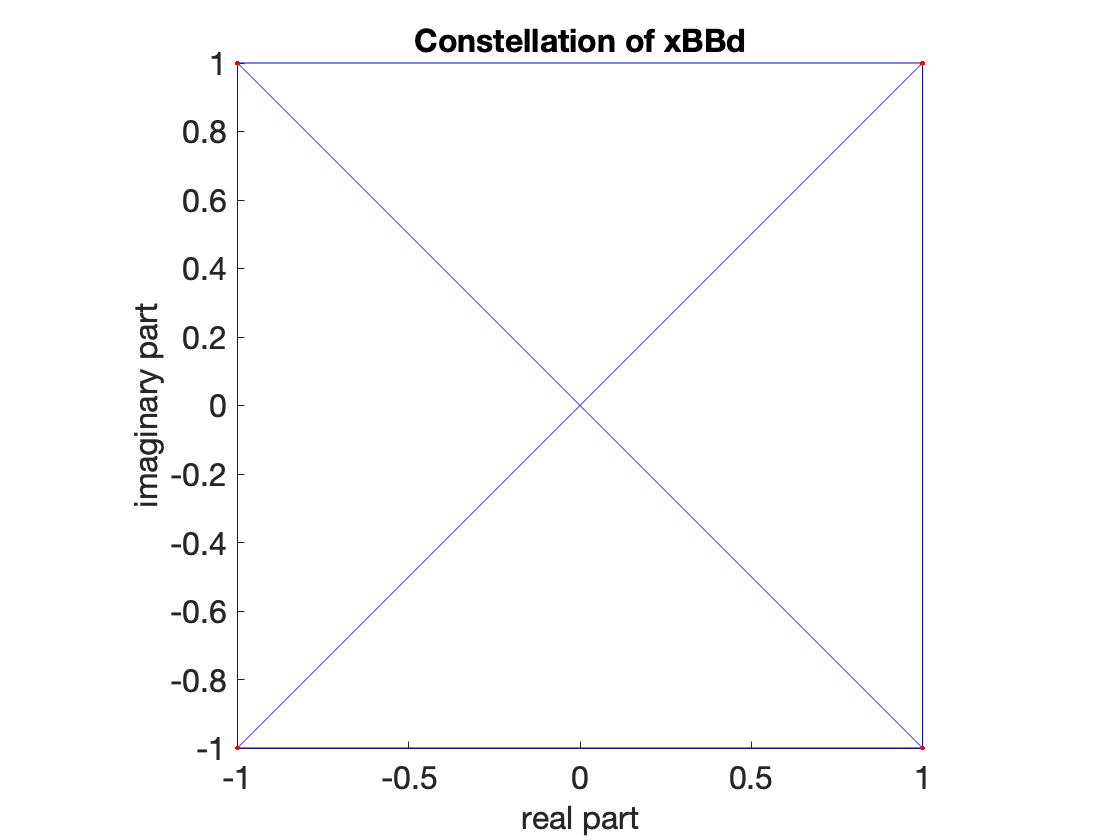
\includegraphics[scale=0.4]{figures/timing-phase-corrected-xrf9.png}
    \caption{Payload of xRF9.mat with Decision Directed Timing Phase Recovery}
    \label{fig:with-dd}
\end{figure}